\subsubsection{\acl{pu} approximation}\label{subsec:pu_approximation}

\citet{chuang_debiased_2020} assume a \acf{pu} learning scenario, 
where positive samples and an unlabelled image dataset $p$ are available.
Since positive samples may not be available in reality, 
the positive distribution $p^+$ is mimicked by data augmentations.

\citeauthor{chuang_debiased_2020}'s goal is to sample \acp{tn}.
They denote sampling bias as the phenomenon of sampling \acp{fn} as illustrated in \autoref{fig:sampling_bias}a.
When randomly sampling negative samples from the data distribution $p$ 
a negative sample can inherently belong to the same class as the anchor.
The negative effect of sampling bias on the model's performance is illustrated in \autoref{fig:sampling_bias}b. % intuition
Consequently, they propose a debiased contrastive objective that corrects for sampling \acp{fn} 
%i.e., the selection of negative samples that have the same label as the anchor, 
in an unsupervised scenario.
The idea is to generate positive samples using augmentations,
to sample negative samples $x^-$ from the data distribution $p$
and to add a correction term for \acp{fn} in the loss function. 
% why and how does correction term work?
The correction term is a factor in the divisor of the loss and 
essentially down-weights the contribution of negative pairs that are likely to be \acp{fn}. 
% TODO: necessary how likely is defined? dot product of representations
This prevents the model from penalizing these pairs too heavily and 
allows the positive samples to remain close in the embedding space, 
thereby improving the learned representation by maintaining the proximity of True Positives.

\begin{figure}%
    \centering
    \subfloat[\centering Visualization of sampling bias similar to \citet{chuang_debiased_2020}. Sampling $x_i^-$ from $p$ can result in \ac{fn}.]
    {{\includegraphics[width=5cm]{images/sampling_bias.png} }}%
    \qquad
    \subfloat[\centering Negative influence of sampling bias on accuracy from \citet{chuang_debiased_2020}.]{{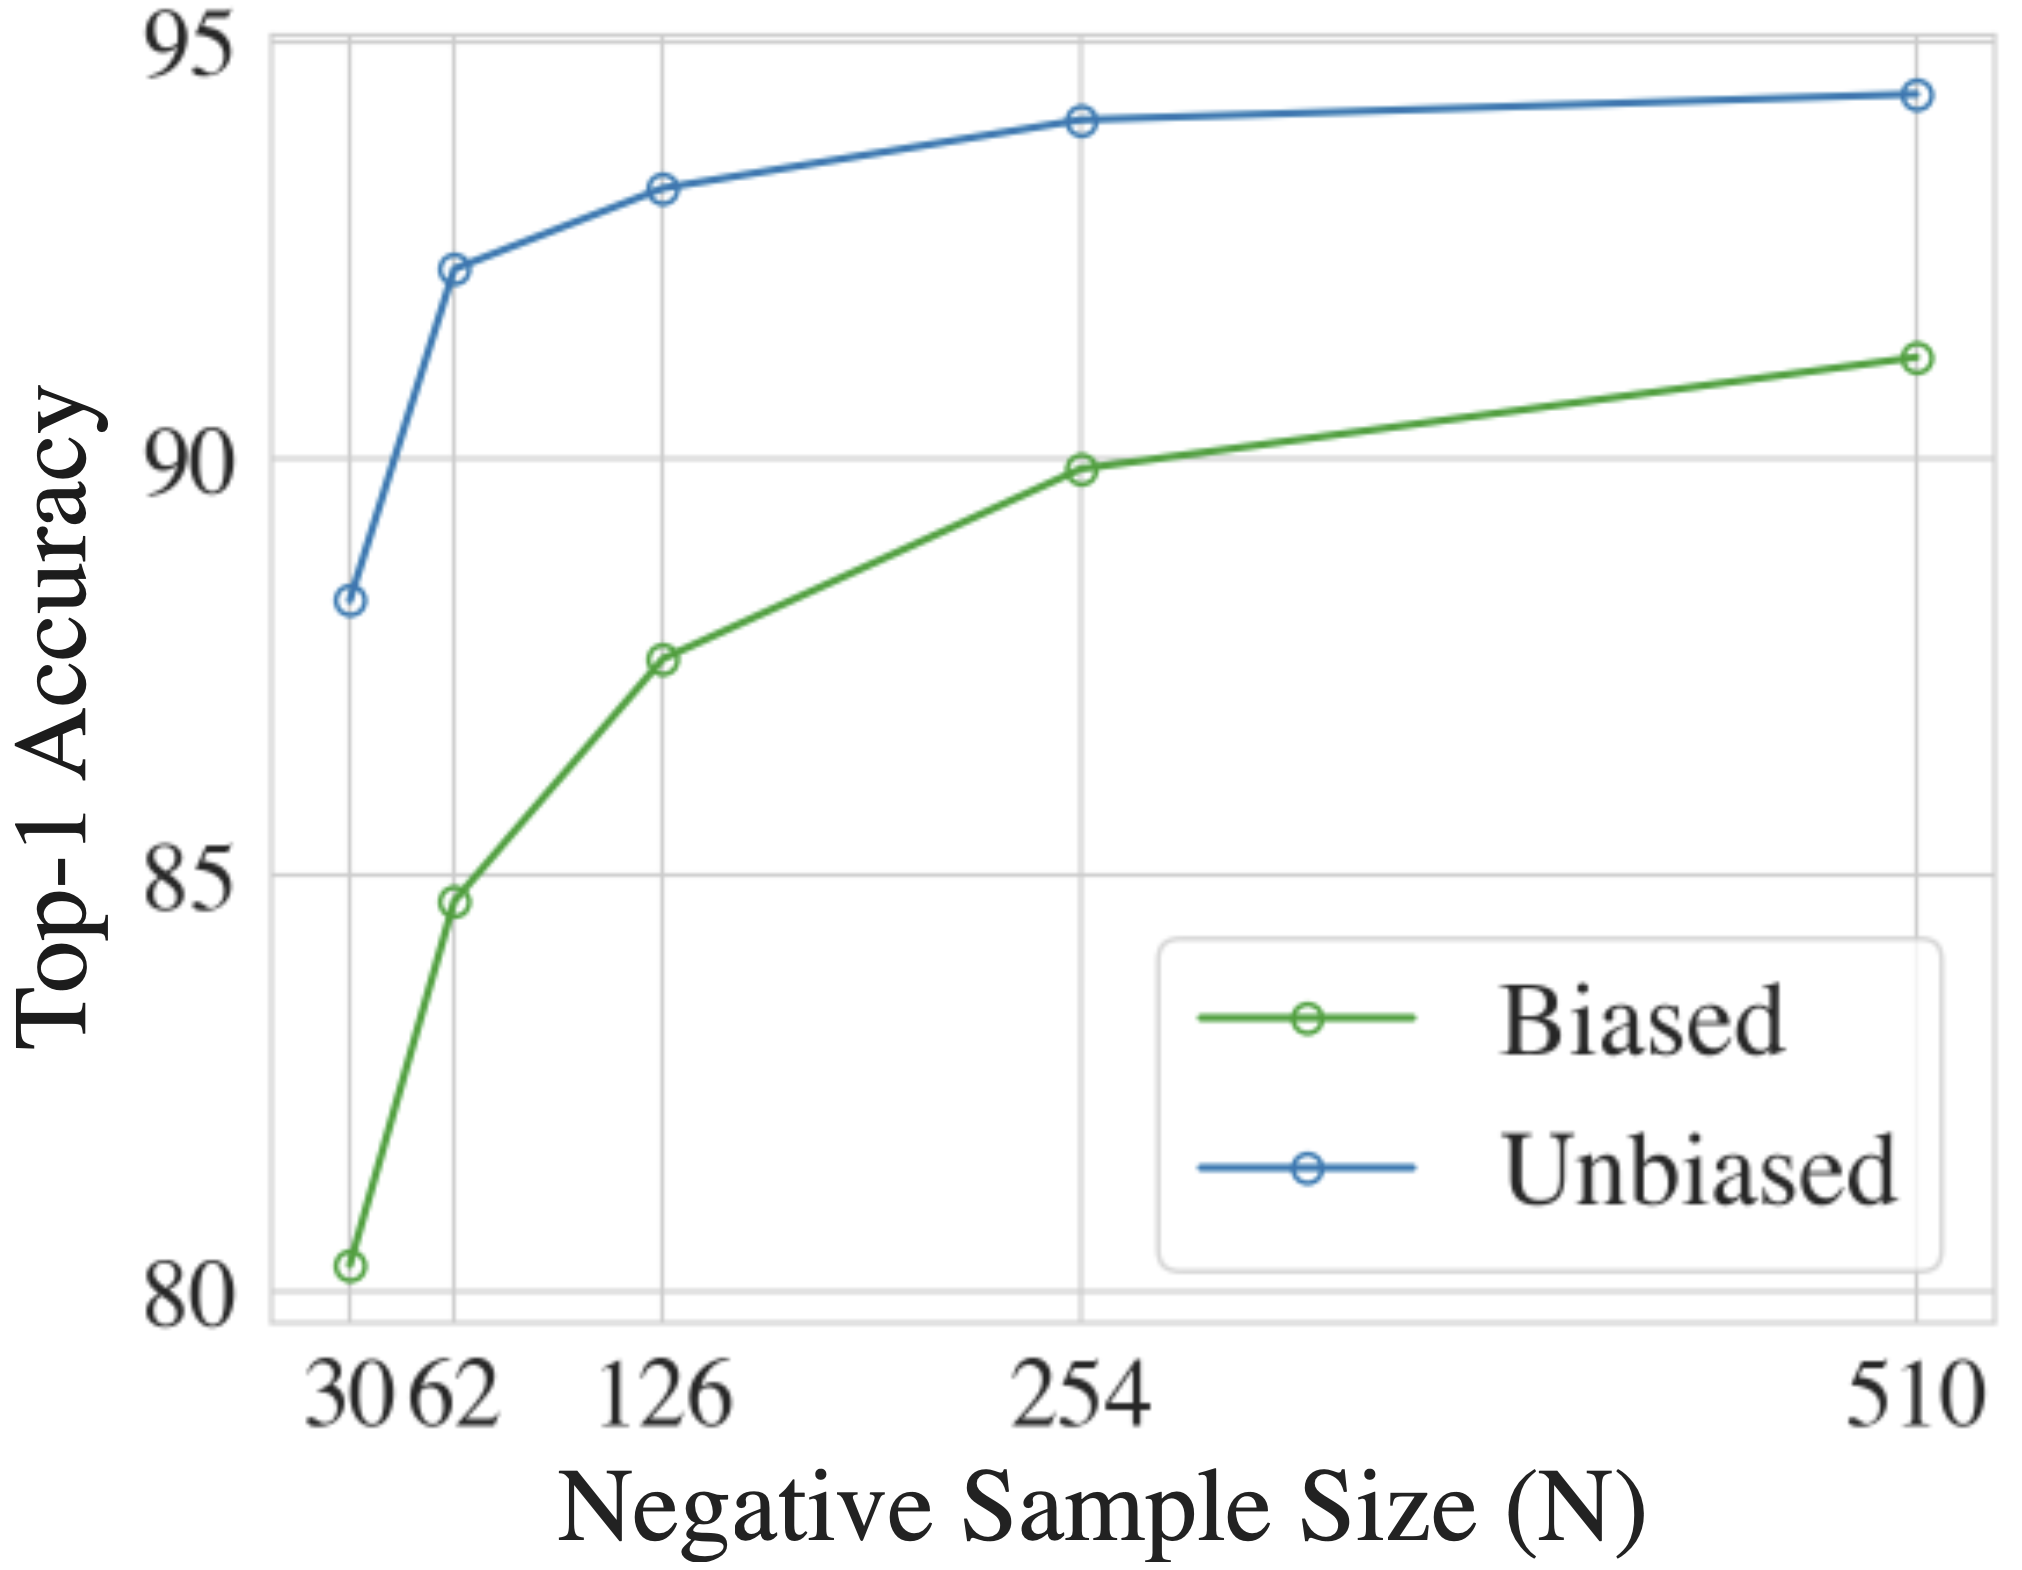
\includegraphics[width=5cm]{images/debiased_sampling_accuracy.png} }}%
    \caption{Visualization of sampling bias and its effect on the model's performance.}%
    \label{fig:sampling_bias}%
\end{figure}